\documentclass{article}  
\usepackage{array}
% Include all project wide packages here.
\usepackage{fullpage}
\usepackage{polyglossia}
\setmainlanguage{english}
\usepackage{csquotes}
\usepackage{graphicx}
\usepackage{epstopdf}
\usepackage{pdfpages}
\usepackage{caption}
\usepackage[list=true]{subcaption}
\usepackage{float}
\usepackage{standalone}
\usepackage{import}
\usepackage{tocloft}
\usepackage{wrapfig}
\usepackage{authblk}
\usepackage{array}
\usepackage{booktabs}
\usepackage[toc,page,title,titletoc]{appendix}
\usepackage{xunicode}
\usepackage{fontspec}
\usepackage{pgfplots}
\usepackage{SIunits}
\pgfplotsset{compat=newest}
\pgfplotsset{plot coordinates/math parser=false}
\newlength\figureheight 
\newlength\figurewidth
\usepackage{unicode-math}
\usepackage[
    backend=bibtexu,
	texencoding=utf8,
bibencoding=utf8,
    style=ieee,
    sortlocale=nl_NL,
    language=auto
]{biblatex}
\usepackage{listings}
\newcommand{\includecode}[3][c]{\lstinputlisting[caption=#2, escapechar=, style=#1]{#3}}
\newcommand{\superscript}[1]{\ensuremath{^{\textrm{#1}}}}
\newcommand{\subscript}[1]{\ensuremath{_{\textrm{#1}}}}


\newcommand{\chapternumber}{\thechapter}
\renewcommand{\appendixname}{Bijlage}
\renewcommand{\appendixtocname}{Bijlagen}
\renewcommand{\appendixpagename}{Bijlagen}

\usepackage[hidelinks]{hyperref} %<--------ALTIJD ALS LAATSTE
  
\renewcommand{\familydefault}{\sfdefault}

\setmainfont[Ligatures=TeX]{Myriad Pro}
\setmathfont{Asana Math}
\setmonofont{Lucida Console}

\usepackage{titlesec, blindtext, color}
\definecolor{gray75}{gray}{0.75}
\newcommand{\hsp}{\hspace{20pt}}
\titleformat{\chapter}[hang]{\Huge\bfseries}{\chapternumber\hsp\textcolor{gray75}{|}\hsp}{0pt}{\Huge\bfseries}
\renewcommand{\familydefault}{\sfdefault}
\renewcommand{\arraystretch}{1.2}
\setlength\parindent{0pt}

%For code listings
\definecolor{black}{rgb}{0,0,0}
\definecolor{browntags}{rgb}{0.65,0.1,0.1}
\definecolor{bluestrings}{rgb}{0,0,1}
\definecolor{graycomments}{rgb}{0.4,0.4,0.4}
\definecolor{redkeywords}{rgb}{1,0,0}
\definecolor{bluekeywords}{rgb}{0.13,0.13,0.8}
\definecolor{greencomments}{rgb}{0,0.5,0}
\definecolor{redstrings}{rgb}{0.9,0,0}
\definecolor{purpleidentifiers}{rgb}{0.01,0,0.01}


\lstdefinestyle{csharp}{
language=[Sharp]C,
showspaces=false,
showtabs=false,
breaklines=true,
showstringspaces=false,
breakatwhitespace=true,
escapeinside={(*@}{@*)},
columns=fullflexible,
commentstyle=\color{greencomments},
keywordstyle=\color{bluekeywords}\bfseries,
stringstyle=\color{redstrings},
identifierstyle=\color{purpleidentifiers},
basicstyle=\ttfamily\small}

\lstdefinestyle{c}{
language=C,
showspaces=false,
showtabs=false,
breaklines=true,
showstringspaces=false,
breakatwhitespace=true,
escapeinside={(*@}{@*)},
columns=fullflexible,
commentstyle=\color{greencomments},
keywordstyle=\color{bluekeywords}\bfseries,
stringstyle=\color{redstrings},
identifierstyle=\color{purpleidentifiers},
}

\lstdefinestyle{matlab}{
language=Matlab,
showspaces=false,
showtabs=false,
breaklines=true,
showstringspaces=false,
breakatwhitespace=true,
escapeinside={(*@}{@*)},
columns=fullflexible,
commentstyle=\color{greencomments},
keywordstyle=\color{bluekeywords}\bfseries,
stringstyle=\color{redstrings},
identifierstyle=\color{purpleidentifiers}
}

\lstdefinestyle{vhdl}{
language=VHDL,
showspaces=false,
showtabs=false,
breaklines=true,
showstringspaces=false,
breakatwhitespace=true,
escapeinside={(*@}{@*)},
columns=fullflexible,
commentstyle=\color{greencomments},
keywordstyle=\color{bluekeywords}\bfseries,
stringstyle=\color{redstrings},
identifierstyle=\color{purpleidentifiers}
}

\lstdefinestyle{xaml}{
language=XML,
showspaces=false,
showtabs=false,
breaklines=true,
showstringspaces=false,
breakatwhitespace=true,
escapeinside={(*@}{@*)},
columns=fullflexible,
commentstyle=\color{greencomments},
keywordstyle=\color{redkeywords},
stringstyle=\color{bluestrings},
tagstyle=\color{browntags},
morestring=[b]",
  morecomment=[s]{<?}{?>},
  morekeywords={xmlns,version,typex:AsyncRecords,x:Arguments,x:Boolean,x:Byte,x:Char,x:Class,x:ClassAttributes,x:ClassModifier,x:Code,x:ConnectionId,x:Decimal,x:Double,x:FactoryMethod,x:FieldModifier,x:Int16,x:Int32,x:Int64,x:Key,x:Members,x:Name,x:Object,x:Property,x:Shared,x:Single,x:String,x:Subclass,x:SynchronousMode,x:TimeSpan,x:TypeArguments,x:Uid,x:Uri,x:XData,Grid.Column,Grid.ColumnSpan,Click,ClipToBounds,Content,DropDownOpened,FontSize,Foreground,Header,Height,HorizontalAlignment,HorizontalContentAlignment,IsCancel,IsDefault,IsEnabled,IsSelected,Margin,MinHeight,MinWidth,Padding,SnapsToDevicePixels,Target,TextWrapping,Title,VerticalAlignment,VerticalContentAlignment,Width,WindowStartupLocation,Binding,Mode,OneWay,xmlns:x}
}

%defaults
\lstset{
basicstyle=\ttfamily\small,
extendedchars=false,
numbers=left,
numberstyle=\ttfamily\tiny,
stepnumber=1,
tabsize=4,
numbersep=5pt
}  
\begin{document}


LIDAR is an acronym for Light Detection and Ranging. It is a technique that uses a laser beam to detect or scan objects. It is an active form of remote sensing. So information is obtained by sending a signal from a transmitter which can be reflected by a target. A detector can pick up the reflected signal to determine different types of information about the object. These types are range, chemical properties and velocity.
In our case we are only interested in the range of the object, since our goal is to avoid collisions with static objects. The measurement of the range or distance of the object is based on a precise measurement of time. There are two main methods to do this, the timed pulse method and the phase comparison method.


\subsubsection{Timed Pulse Method}

As the name indicates, the timed pulse method measures the time required for a very short pulse of laser radiation to travel to the target and back. This method can be used to measure distances of tens of meters to hundreds of kilometers. In figure \ref{lidar1} is the generic type of a laser rangefinder shown, of course the actual design and the specific components that will be used in a particular instrument will depend on the particular application. In our case the laser will be a small low-powered laser instead of a high-powered one.

\begin{figure}[H]
	\centering
	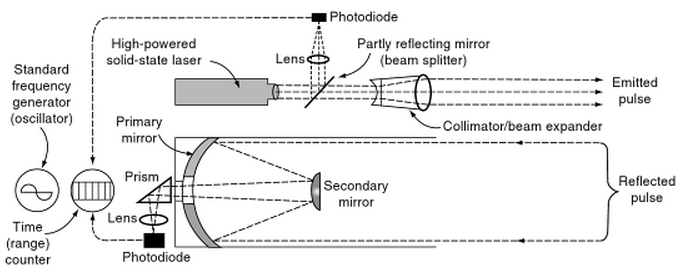
\includegraphics[scale=0.8]{figures/TimedPulse}
	\caption{Laser rangefinder. }
	\label{lidar1}
\end{figure}

A lens is placed in front of the laser to first expand and then collimate the laser pulse so the divergence is kept to a minimum. A small part of the energy of an emitted pulse will be diverted by a partly reflecting mirror to a photodiode. This will trigger a timing device with a simple threshold which is usually connected to a very stable oscillator. When the pulse is reflected from the object the returning pulse is picked up by the receiving lens or mirror optics. Because the pulse will collide with the object and tiny particles in the air, the beam will be scattered and very weak in intensity compared to the sent laser pulse. Therefore it is needed to amplify the returned pulse electrically after it has been picked up by a sensitive photodiode. To reduce the noise picked up by this photodiode (e.g. sunlight) 
narrowband optical filters are placed over it. In simple cases, this picked up reflected pulse will deliver a stop pulse to the timer counter. When this stop pulse reaches a certain threshold the counter will be stopped. When more state-of-the-art systems are used, a more complex triggering mechanism is used of course. Since the time it took for the sent pulse to travel to the object and back is now known, the distance can be calculated using the speed of light.

\subsubsection{Phase Comparison Method}

In contrast to the timed pulse method, a continuous laser beam is used in the phase comparison method. A continuous laser beam is often abbreviated to CW laser, which stands for continuous wave laser.Because of the limited power of a CW laser it is almost never used for long range systems. On the other hand, this makes it very suitable for measuring shorter distances (typically \textless 100m). In the phase comparison method, the emitted beam is a basic carrier signal on which a modulation signal has been superimposed. This modulation signal is used to measure the difference in phase of the transmitted and received signal. The frequency of the modulation signal is held at a constant value using a stable oscillator. This means the modulation wave can be used to control the amplitude of the carrier wave, which is known as amplitude modulation. A picture of the modulation process is shown in figure \ref{lidar2}. 


\begin{figure}[H]
	\centering
	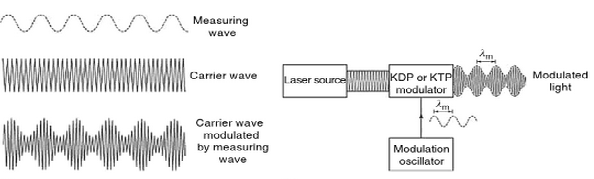
\includegraphics[scale=1]{figures/Modulation}
	\caption{Amplitude modulation. }
	\label{lidar2}
\end{figure}


In the phase comparison method the emitted CW laser is also reflected by an object it collides with. This means a small part of the emitted beam will be reflected and will travel back through the same path as the emitted beam. Just like the timed pulse method the reflected signal is detected using a photodiode and amplified. After amplification the signal will be demodulated, this means the carrier and the modulation signal will be separated. Now the phase of reflected signal is compared to the original emitted signal, from this the phase angle between the two signals can be obtained. The graphs in figure \ref{lidar3} show how the transmitted signal is reflected by an object and picked up by the receiver (a), and how the phase angle is determined between the transmitted and received signal (b). 



\begin{figure}[H]
	\centering
	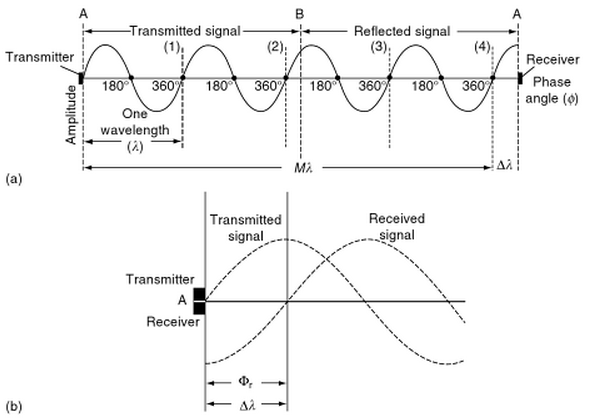
\includegraphics[scale=0.8]{figures/Phaseangle}
	\caption{Phase angle measurement method }
	\label{lidar3}
\end{figure}

The phase angle is the fractional part of the total distance.The total distance consists of an integer number multiplied by the wavelength plus the fractional part. This is also shown in graph (a). So the total distance measured can be calculated using the following formula:

\begin{equation}
d = (M \lambda + \delta \lambda)
\end{equation}

The integer M can be determined by making a number of changes to the wavelength, which in turn changes the frequency of the emitted beam. By doing this very rapidly in succession a system of equations is generated that can be solved for the final distance d.

\end{document}